\documentclass[UTF8]{ctexart}
\usepackage{subfiles}  

%下面的语句, 引入你的头部设置文件
\usepackage{C:/phpStorm_proj/02_myself_ID_EGO/+100_latex_all_math_sel/myPreamble} 
%必须是绝对路径，才能让各个tex在单独编译时使用到

\title{向量组的线性相关性}


%---------------------------------


\begin{document}
\tableofcontents % 生成目录
\date{} % 若不写这句, 则默认也会渲染出日期, 所以我们要手动赋空值
\maketitle  %这行代码, 让你前面的 title, author, date生效

\section{向量 vector 的几何意义}

\subsection{向量, 就是箭头线段的``终点"坐标}

通常, 当你考虑``一个"向量时, 就把它看成是``箭头". \\
当你考虑``多个"向量时, 就把它看成是``箭头终点"的那个点(point).\\

\textbf{注意: 向量的值, 表示的是坐标轴的位置, 而不是该向量线段的长度(即不是`模"的概念).}\\


\includegraphics[width=0.4\textwidth]{img/0066.png}\\


\textbf{向量没有确定的位置, 它们不依赖于任何坐标系而存在。} 所以, 凡是两个向量大小相等、方向相同的，我们就说这两个向量是相等的。\\

虽然向量独立于任何坐标系之外，但为了与解析技术联系起来, 以实现对向量的计算，数学上, 我们还必须把向量放在某一个坐标系下来研究。\\
如果把空间中所有的向量的尾部, 都拉到坐标原点，这样, n维点空间, 就可以与n维向量空间, 建立起一一对应的关系: n维点空间中的点(0,0,0，...)取作原点，那么\textbf{每一个点, 都可以让一个向量和它对应.} 这个向量就是``从坐标原点出发, 到这个点为止的向量"。\\
\textbf{我们默认所有的向量是``从原点出发"的，不要忘了这个约定。}\\



向量, 被看做线性空间, 或向量空间中的一个元素。但向量与点不同，\textbf{向量表示的是``两点之间的位移", 而不``是空间中的物理位置"，它是独立于坐标系的. 这就是为什么我们可以在描述向量的加法、数乘等运算的几何解释时, 常常不用画出坐标系}，但一个点离开坐标系就无法表示. 向量还可以``确定方向", 而一个点就不能。\\



~\\
\hrule
~\\

\subsection{向量的加法 → 平行四边形法则}

把单位坐标向量 i(1,0,0), j(0,1,0), k(0,0,1) 首尾连接相加，就得到了(1,1,1)的图像. \\

\includegraphics[width=0.8\textwidth]{img/0122.png}\\

所以, 任意一个向量 a=(x,y,z), 就可以表示为 a=(x,y,z)=xi+yi+zk.  (← x,y,z是系数倍). 即分别对``单位坐标向量" 进行缩放x、y、z倍, 然后相加.\\

\includegraphics[width=0.5\textwidth]{img/0123.png}\\

向量的运算, 有: \\
- 加法 \\
- 减法 \\
- 乘法(包括两种: 点积, 叉积). 
- 但没有除法. \\


\begin{myEnvSample}
把 u, v, w, a 四个向量相加, 得到的结果(新向量), 就是``从原点出发, 直接指向最后一个向量a的尾部"的b向量.	\\

\includegraphics[width=0.5\textwidth]{img/0124.png}
\end{myEnvSample}

多个向量加法的本质, 实际上是这些向量, 在坐标轴上的投影的合成(相加或相减)后的结果. 同样, 点积和叉积, 也是这个数学结果的体现. \\

\includegraphics[width=0.5\textwidth]{img/0125.png}\\





~\\
\hrule
~\\

\subsection{向量的``数乘" : 系数k的作用, 是把向量伸缩 k倍}

$2\left| \begin{array}{l}
		x \\
		y \\
	\end{array} \right|=\left| \begin{array}{l}
		2x \\
		2y \\
	\end{array} \right|
$\\


\includegraphics[width=0.4\textwidth]{img/0067.png}\\
\\


$text{其充要条件是:\ 要么\ 数}k=0,\ \text{或要么\ }\alpha =0\text{向量}$


~\\
\hrule
~\\








\subsection{单位向量 : 基 basis}

The \textbf{basis} of a vector space /is a set of linearly independent vectors /that span the full space.


\includegraphics[width=0.6\textwidth]{img/0068.png}\\

$\left. \begin{array}{r}
		\hat{i} = 1 \\
		\hat{j} = 1 \\
	\end{array} \right\}$ ← 称为``单位向量"或``基"\\

事实上, 每当我们描述一个向量时, 它都依赖于我们正在使用的``基".\\

$\vec{v}=\left| \begin{array}{l}
		3  \\
		-2 \\
	\end{array} \right|= 3 \hat{i} + (-2)\hat{j}$\\


\includegraphics[width=0.3\textwidth]{img/0069.png}\\

向量的终点坐标, 其实就是系数倍的``基向量"的线性组合.\\



【你可以选择任意两个方向作为``基", 只要它们互相垂直即可.】 \\
比如，你可以选择指向右上方的向量 v, 和 指向右下方的向量 w, 作为基向量. \\
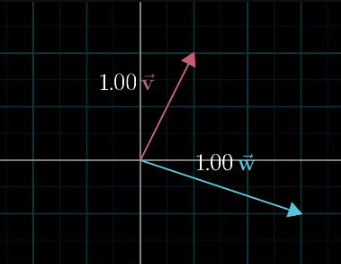
\includegraphics[width=0.35\textwidth]{img/0102.png}\\

这组新的基向量, 进行缩放, 再相加，同样能构造出其他的向量.\\
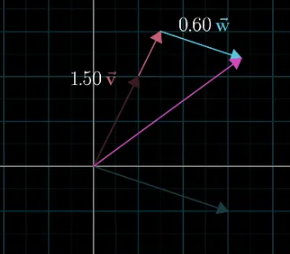
\includegraphics[width=0.35\textwidth]{img/0103.png}\\

所以, 一组``基向量", 就对应一个坐标系. 选择不同的基向量, 就构造出了不同的坐标系. 同一个向量，在不同的坐标系下(即采用不同的基向量)，其坐标值也要相应地发生变化. \\

上面, 反复出现\textbf{``将向量进行缩放,再相加"的操作, 这样的操作，我们称之为``线性组合".}


~\\
\hrule
~\\

\subsection{张成 span}

【二维空间中】:\\
在二维平面中，选取 2 个向量, ，然后考虑它们所有可能的``线性组合", 我们会得到什么呢? 这取决于我们选择的 2 个向量.\\

→ 通常情况下，我们会得到整个平面.\\
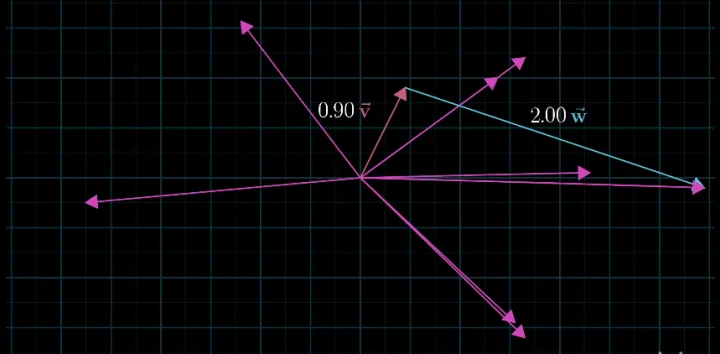
\includegraphics[width=0.7\textwidth]{img/0104.png}\\

→ 但如果选择的 2 个向量，恰好``共线"的话，那它们的线性组合, 就被局限在一条过原点的直线上了. \\
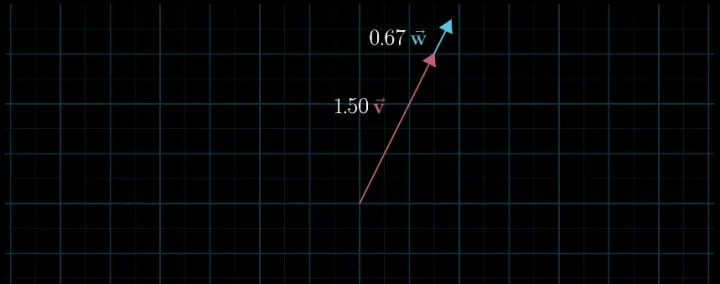
\includegraphics[width=0.7\textwidth]{img/0105.png}\\

→ 最极端的情况是，如果选择的 2 个向量都是零向量，那么它们的线性组合, 就只可能是零向量了. \\
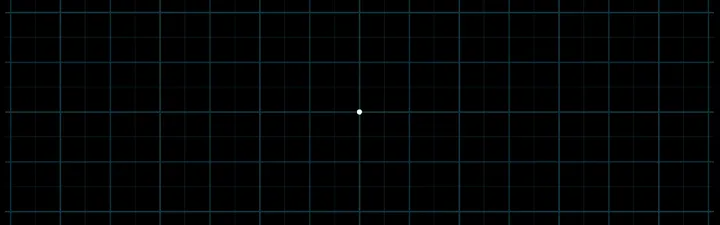
\includegraphics[width=0.7\textwidth]{img/0106.png}\\

``数乘"和``加法", 是向量的两个最基础的运算. \textbf{当我们谈论向量所``张成"的空间时，我们实际上就是在问: 仅仅通过``数乘"和``加法''这两种运算，你能获得的所有可能的向量集合是什么.} \\

在线性代数中，向量的起点, 始终固定在``原点"的位置，因此, 向量的终点就唯一确定了向量本身. 这样，我们便可以将向量, 看成是``空间中的点"（即``向量的终点"）.\\


【三维空间中】:\\
将线性组合的想法扩展到 3 维空间中。想象 3 个 三维向量，它们所张成的空间会是什么样的呢？这取决于我们选择的 3 个向量的箭头位置:\\

→ 通常情况下，我们会得到整个 3 维空间. \\
→ 当选择的 3 个向量是``共面"时(即3个向量, 存在在两个维度的世界上)，它们所张成的空间, 就是一个过``原点"的二维平面. \\
→ 当 3 个向量``共线"时(即3个向量, 共同挤在一个维度上)，它们所张成的空间, 就是一条过原点的一维直线. \\
→ 当 3 个向量都是零向量时 (即三个向量, 都挤在0维度的世界上)，它们所张成的空间, 就只扩展到零向量 .\\

\textbf{显然, 在满足能够``张成"一个空间时, 只需要最低的维度数量就行了. 比如张成2维空间, 只需要最低2个向量(即轴)就行了. 用3个向量去``张成"二维空间, 那其中有 1 个向量是多余的.  数学上，我们就是用 \hypertarget{超链接定位符}{``线性相关"}来描述这样的``多余向量"的现象.}  \\

→ \textbf{当我们说: ``几个向量所构成的向量组, `线性相关'"时，意思就是说: 向量组中的 (任意) 一个向量, 都可以用``向量组"中其他向量的``线性组合", 来表示出来。也就是说: 这个向量, 已经落在其他向量所``张成"的空间中，它对整个向量组张成的空间是没有贡献的，把它从``向量组"中拿掉，并不会影响向量组所张成的空间的维度 (即空间维度不会塌缩, 不会降维). \\}
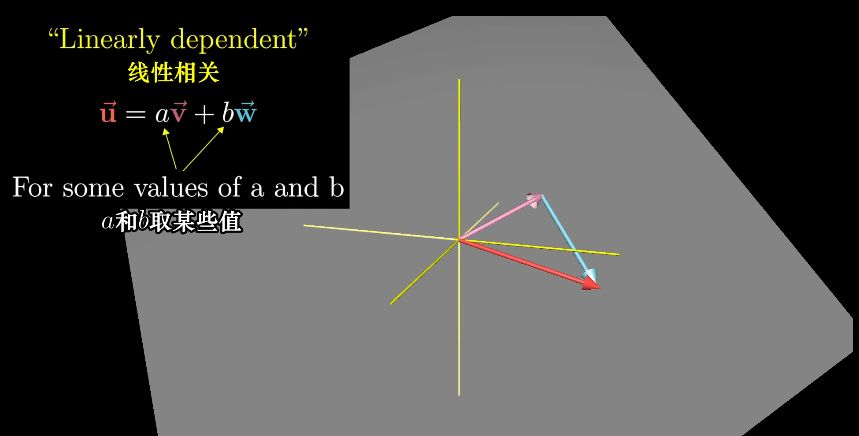
\includegraphics[width=0.6\textwidth]{img/0107.png}\\

→ 那么\textbf{``线性无关"就指的是: 向量组中的（任意）一个向量, 都无法用``该向量组"中其他向量的``线性组合"来表示出来。换句话说: 向量组中的每一个向量, 都为该向量组所张成的空间贡献了一个维度(一个轴). 少了任何一个向量，都会让空间降维.}\\
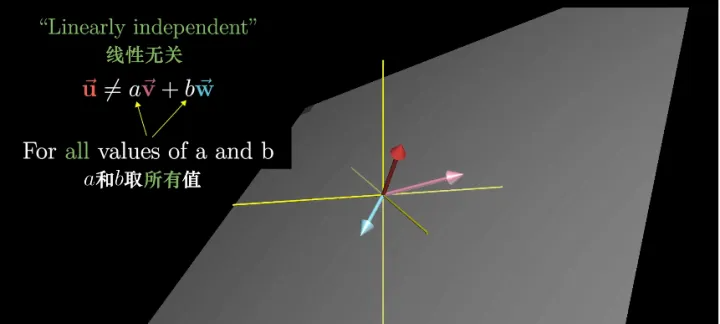
\includegraphics[width=0.6\textwidth]{img/0108.png}\\


\textbf{所以: 向量空间的一组``基"(即维度, 轴), 就是``张成"该空间的一个``线性无关"的``向量集".} The basis of a vector space /is a set of linearly independent vectors /that span the full space. \\





the span of $\vec{v}$ and $\vec{w} $  /is the set of  all their linear combinations.\\
the set of all possible vectors /than you can reach /is called the span of those two vectors. ← 相当于``势力范围", 就是张成.\\


两个斜率不同的向量(a,b), 自由伸缩, 它们的和(即a+b=c), 即新向量c的终点, 能遍及二维平面上的任何点处.\\


\includegraphics[width=0.6\textwidth]{img/0070.png}\\

但如果两个向量都是``零向量"的话, 它们的系数倍的和, 也永远被束缚在原点(0,0)了. $ k_1 \vec{0}  +  k_2 \vec{0}=0$ \\

三维空间中, 两个斜率同的向量, 能``张成"出``过原点"的一个平面.\\

\includegraphics[width=0.4\textwidth]{img/0071.png}\\

三维空间中, 三个斜率不同的向量, 它们的和, 能张成出三维空间中所有的地方. \\
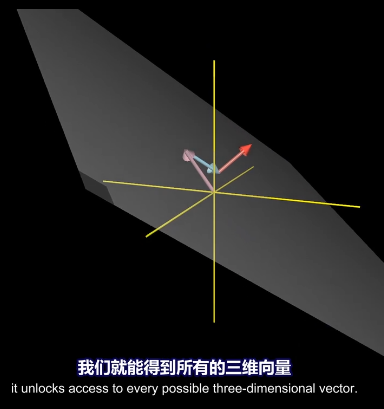
\includegraphics[width=0.4\textwidth]{img/0072.png}\\


~\\
\hrule
~\\
\section{向量的点积 (内积) : $x \cdot y = x_{1} y_{1} + x_{2} y_{2} + ...$}

向量的内积, 也叫数量积、标积、点积. 因为``内积"的结果就是个``数量"或者``标量 scalar".\\

【标量】:\textbf{只具有数值大小，而没有方向} (部分有正负之分). \\
标量（或作纯量）是指在``坐标变换"下保持不变的物理量。如: 质量、密度、温度、功、能量、路程、速率、体积、时间、热量、电阻、功率、势能、引力势能、电势能等物理量。\textbf{无论选取什么坐标系，``标量"的数值恒保持不变。}\\

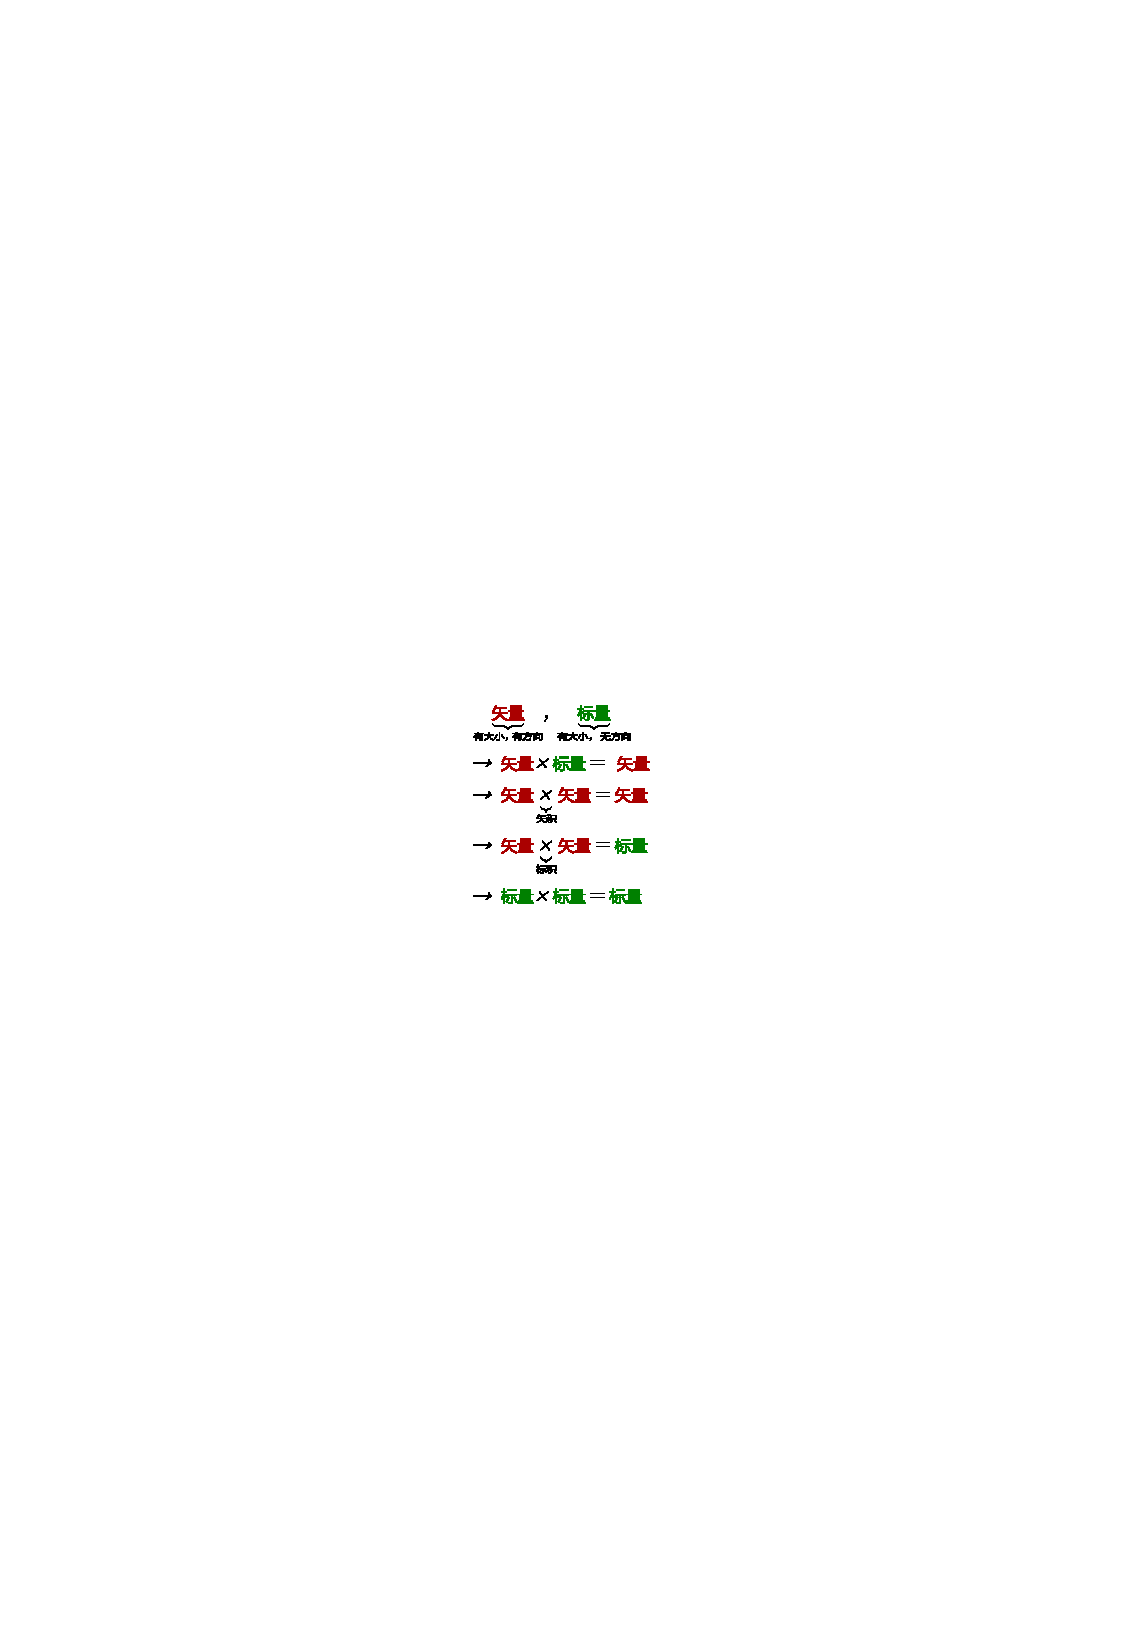
\includegraphics[width=0.25\textwidth]{img/0126.pdf}\\

\textbf{``矢量加法"一般可用平行四边形法则。但``标量加法"不遵守平行四边形法则！}\\


【向量(矢量)的内积, 有两种定义】:  \\
(1): $ \boxed{
a\cdot b=ab\cdot \cos \theta 
}$  ← 就是说, 等于 向量 a, b 的长度之积, 再乘以它们夹角的余弦. \\

(2): $\boxed{
	\overrightarrow{a}\cdot \overrightarrow{b}=a_xb_x+a_yb_y+a_zb_z
	}$ ← 即等于 先让两个向量对应的``分量", 做相乘, 然后再把这些乘积做求和. \\


\begin{myEnvSample}
上面这两个公式, 其实是一回事. 你可以这样来理解: \\
你有一个向量a, 现在,你来创建一个这样的坐标系: 让坐标系的原点, 和向量a的起点重合; 让坐标系的x轴, 重合于向量a的箭头方向. \\
则, 用这个坐标系, 来衡量向量a的箭头端点处的坐标, 就是: $
\overrightarrow{a}=\left| \begin{array}{l}
	a_x\\
	a_y\\
	a_z\\
\end{array} \right|=\left| \begin{array}{l}
	a\\
	0\\
	0\\
\end{array} \right|
$\\

那么, 我们就来看看, ``a向量"和``另一个向量b"的点积, 会是什么? \\
$
\overrightarrow{a}\cdot \overrightarrow{b}=\underset{=a}{\underbrace{a_x}}b_x+\underset{=0}{\underbrace{a_y}}b_y+\underset{=0}{\underbrace{a_z}}b_z=a\cdot \underset{\text{即}b\text{在}x\text{轴上的坐标值}}{\underbrace{b_x}}
$\\

注意: $b_x$ 是向量b在x轴上的分量值, 而x轴就是``向量a"所在的方向. 所以 $b_x$ 就是b在a上的投影了! 而 $
\cos \theta =\frac{b_x}{\overrightarrow{b}},\ \text{即\ }b_x=b\cdot \cos \theta 
$\\

所以, $
\overrightarrow{a}\cdot \overrightarrow{b}=a\cdot \underset{=b\cdot \cos \theta}{\underbrace{b_x}}=a\cdot b\cdot \cos \theta 
$ ← 到此, 点积的两个公式, 就统一起来了. 


\includegraphics[width=0.55\textwidth]{img/0127.png}\\

\textbf{因此,向量``内积"的几何解释, 就是一个向量在另一个向量上的投影的积, 也就是同方向的积.}
\end{myEnvSample}


特别地，\textbf{如果一个向量(如量a)是某个坐标轴的``单位坐标向量". 那么，两个向量的内积 $a \cdot b$ , 就是向量b在此坐标轴上的坐标值。因此，如果想要将一个向量, 变换到新的坐标系上，就只需进行``内积"运算即可。}这个结论很重要，这是``傅立叶分析"的理论基础之一。\\

实际上,\textbf{ 矩阵的乘法运算, 就是``内积"运算.} 两个矩阵相乘, 就是左矩阵的行（向量）, 与右矩阵的列（向量), 进行逐次内积. \\



【从``内积"值上, 我们还可以看出两个向量在方向上的接近程度】:\\
→ 内积值 > 0 时: 两个向量, 大致指向``相同"的方向 (方向夹角小于90°)\\
→ 内积值 < 0 时: 两个向量大致指向``相反"的方向 (方向夹角大于90°)\\
→ 内积值 = 0 时: 两个向量``互相垂直".\\

笼统来说，\textbf{内积值越大，两个向量在方向上的就越接近; 内积值越小，在方向上就越相反。}\\

比如下图: \\

\includegraphics[width=0.6\textwidth]{img/0128.png}\\
- 向量a 与 $b_1$ 的夹角最小, 方向最接近. 所以它们的内积为正数. \\
- 向量a 与 $b_2$ 的方向垂直, 内积就为0. \\
- 向量a 与 $b_3$ 的夹角为钝角, 方向基本相反, 内积就为负数. \\








~\\
\hrule
~\\



\subsection{点积的几何意义: $\vec{v} \cdot \vec{w} = \vec{v} \cdot \vec{w'}$ ← 其中,$\vec{w'}$ 是 $\vec{w}$ 在 $\vec{v}$ 上的投影长度. }

→ 如果 $\vec{w'}$ 是$\vec{w}$ 在 $\vec{v}$ 上的投影长度.\\
则:  $\vec{v} \cdot \vec{w} = \vec{v} \cdot \vec{w'}$\\

\includegraphics[width=0.4\textwidth]{img/0091.pdf}\\


→ 如果 $\vec{w}$ 的投影, 是在$\vec{v}$ 的反方向延长线上, 则此时:\\
$\vec{v} \cdot \vec{w} = \vec{v} \cdot \vec{w'} = \text{是负值}$\\
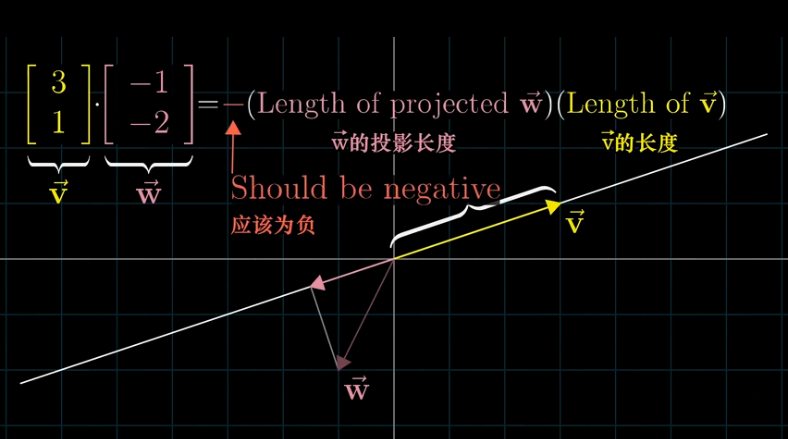
\includegraphics[width=0.6\textwidth]{img/0092.png}\\

→ 如果这两个向量, 本身就互相垂直, 则一个向量在另一个向量上的投影长度, 就为0. 这时它们的``点积"就等于0.\\
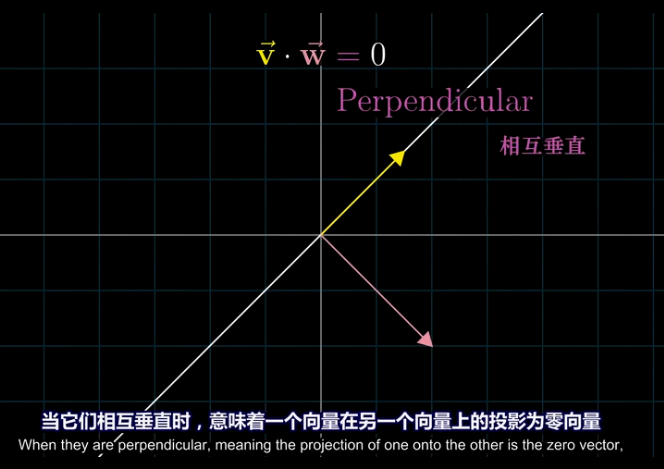
\includegraphics[width=0.5\textwidth]{img/0093.png}\\



\textbf{所以, 注意: ``点积"(inner product)运算的结果, 是一个``数"(投影的长度, 就是一个数呀). 这和向量的其他操作是有区别的.} 比如:  \\
→ 两个向量做``加法", 结果依然是个``向量". \\
→ 向量的``数乘", 结果也依然是个``向量".\\

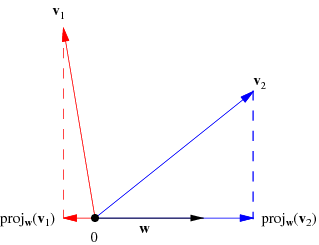
\includegraphics[width=0.4\textwidth]{img/0094.png} \\


\begin{tabular}{|l|l|}
	\hline
	若两个向量 $\vec{x}, \vec{y} $间的夹角 < 90° & $\vec{x} \cdot \vec{y} > 0$              \\
	\hline
	若 $\vec{x}, \vec{y}$ 间的夹角 > 90°         & $\vec{x} \cdot \vec{y} < 0$, 即是个负值. \\
	\hline
	若 $\vec{x}, \vec{y}$ 间的夹角 = 90°         & $\vec{x} \cdot \vec{y} = 0$              \\
	\hline
\end{tabular}





~\\
\hrule
~\\

\subsection{点积的做法公式1 : $ x\cdot y = x_1 y_{1} + x_2 y_{2} + x_{3}y_{3}$}

两个向量的"点积" (inner product  或 dot product 或 scalar product) : $\vec{x} \cdot \vec{y}$, 也有写作 <x,y> 的形式.

点积的做法公式就是:
\begin{align*}
	 & x=\left| \begin{array}{l}
		            x_1 \\
		            x_2 \\
		            x_3 \\
	            \end{array} \right|,\ y=\left| \begin{array}{l}
		                                           y_1 \\
		                                           y_2 \\
		                                           y_3 \\
	                                           \end{array} \right|, \\
	 & \text{则} :
	\boxed{
	\ x\cdot y = x_1 y_{1} + x_2 y_{2} + x_{3}y_{3}
	}
\end{align*}


即:   $x\cdot y = x^T \cdot y$  ← 即把$\vec{x}$横过来, 变成一行, 再和 $\vec{y}$ 的一列相乘. 规则和矩阵的乘法完全一样.\\
其实:   $x\cdot y = x^T \cdot y = y^T  \cdot x$\\

~\\
\hrule
~\\


\subsection{点积的做法公式2: $x \cdot y = \text{x的模} \cdot \text{y的模} \cdot cos \theta$}

两个向量的点积 = 每个向量``模长"的乘积, 再乘以它们的夹角的cos值. \\
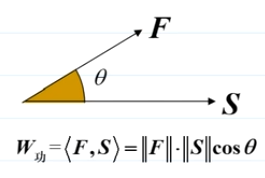
\includegraphics[width=0.25\textwidth]{img/0095.png}\\

根据"余弦定理", 有 : $a^2 = b^2 + c^2 - 2(bc \cdot \cos A) $\\
或: $\cos A = \frac{b^2 + c^2 - a^2} {2bc}$\\

那么对于由两个向量组成的三角形, 如下图, 就有: \\

\includegraphics[width=0.4\textwidth]{img/0096.pdf}



证明过程: \\

\includegraphics[width=0.55\textwidth]{img/0100.pdf}\\



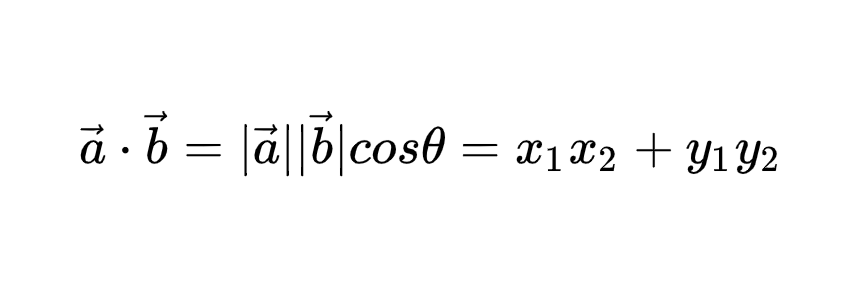
\includegraphics[width=0.4\textwidth]{img/0097.png}
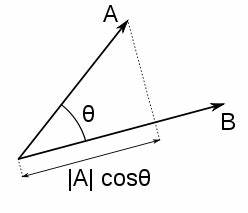
\includegraphics[width=0.2\textwidth]{img/0098.png} \\
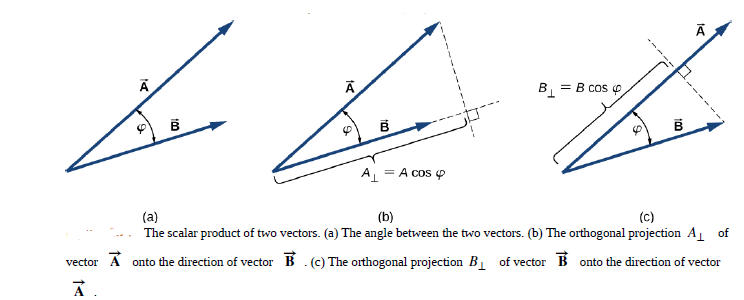
\includegraphics[width=0.9\textwidth]{img/0099.png} \\

根据这个公式, 就可以计算向量a和向量b之间的夹角。从而就可以判断这两个向量是否是同一方向，是否正交(也就是垂直), 等方向关系. 具体对应关系为：\\

~\\
\hrule
~\\




\section{向量的叉积(外积) : $\vec{v} \times \vec{w}$}

向量的 叉积 (外积) exterior product 或  cross product



\subsection{叉积(外积) 的几何意义 : (1)在二维空间中, 是由这两个向量围成的``平行四边形"的面积, 即是一个数值. (2)在三维空间中, 是一个垂直于这个``平行四边形"平面的``新向量".}

【在二维空间中】: \\

\textbf{几何意义上, 叉积, $\vec{v} \times \vec{w}$, 就是由这两个向量围成的``平行四边形"的面积.} \\
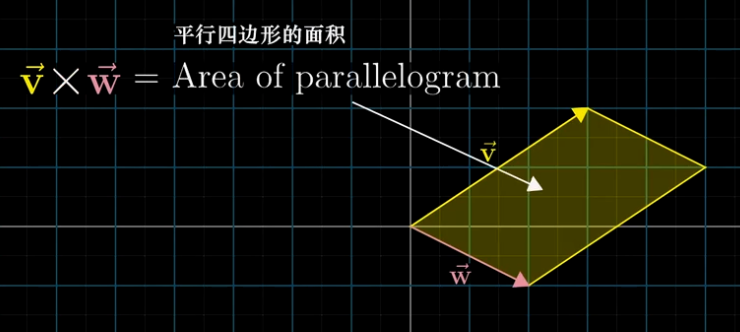
\includegraphics[width=0.5\textwidth]{img/0073.png}\\

\textbf{注意: 顺序会对``叉积"有影响: 如果$\vec{v} \times \vec{w}$ 是正数, 则 $\vec{w} \times \vec{v}$ 就是负数. 即: 交换叉乘时的顺序, 值要变号.} \\

之前说过, 行列式的值, 就是表示的是: 将基 $i \times j$ 的面积, 缩放多少倍.\\
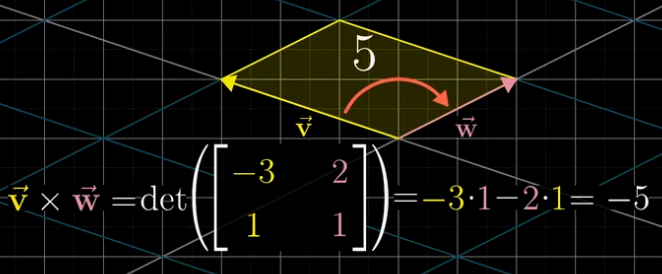
\includegraphics[width=0.5\textwidth]{img/0074.png}\\

面积的概念, 也就证明了: $3(\vec{v} \times \vec{w}) = 3 \vec{v} \times \vec{w}$\\
把平行四边形其中的任一一条边, 延长3倍 , 变成 $3 \vec{v}$ 或  $3 \vec{w}$, 面积也就是 $= 3 (\vec{v} \times \vec{w})$ \\

\includegraphics[width=0.5\textwidth]{img/0075.png}\\




【在三维空间中】:\\
其实, 真正的``叉积", 是通过两个三维向量, 来生成一个新的三维向量. \textbf{注意: 在三维空间中, 叉积的结果不是一个数, 而是一个向量!} \\

\begin{myEnvSample}
	如下面的图中所示, A,B两个箭头的向量的``叉积", 就是第三个向量C. 这个C向量, 始终与两个原点箭头(即A,B)正好为90度.  C向量箭头的长度, 就表示A,B向量的叉积, 它总是完全等于A,B所构成的平行四边形的面积.\\
	
	
\includegraphics[width=0.4\textwidth]{img/0076.png}
	
\includegraphics[width=0.4\textwidth]{img/0077.png}\\
	
\includegraphics[width=0.4\textwidth]{img/0078.png}
	
\includegraphics[width=0.4\textwidth]{img/0079.png}\\
\end{myEnvSample}


\begin{myEnvSample}
	又如: 假设$\vec{v} \times \vec{w} = 2.5$, 在三维空间中, 这两个向量构成一个平面(平行四边形). 它们的``叉积"构成一个新向量 $\vec{p}=2.5$, 它与``平行四边形"所在的面``垂直".\\
	
	
\includegraphics[width=0.7\textwidth]{img/0080.png}\\
	
	即: \textbf{三维叉积, 得到一个三维矢量.}   \\
	\textbf{$\vec{v} \times \vec{w}$得到新的向量$\vec{p}$，新向量$\vec{p}$的长度, 等于向$量\vec{v}$与向量$\vec{w}$组成的平行四边形的面积，并且 向量$\vec{p}$,  与 向量$\vec{v}$ 和向量$\vec{w}$所在平面垂直.}\\
	所以``三维叉积"很容易拿来算平面的``法向量". \\
	
	但垂直于一个平面的向量, 可以有正反两个方向, $\vec{p} $到底是朝哪个方向呢? 这就要用到"右手螺旋法则".\\
	
	
\includegraphics[width=0.7\textwidth]{img/0081.png}
\end{myEnvSample}


~\\
\hrule
~\\

\subsection{右手螺旋法则}

注意顺序: $\vec{a} \times \vec{b} = \vec{c}$, 和 $\vec{b} \times \vec{a} = \vec{c}$, ← $\vec{c}$ 的方向朝向是不同的.

\subsubsection{$\vec{a} \times \vec{b} = \vec{c}$}

1.用右手, 伸展手指, 朝向  $\vec{a}$ \\

\includegraphics[width=0.3\textwidth]{img/0082.png}\\

2.然后, 握拳, 手指收回, 朝向  $\vec{b}$ 的方向. \\

\includegraphics[width=0.3\textwidth]{img/0083.png}\\

3.则, 大拇指朝向的方向, 就是 $\vec{a} \times \vec{b} = \vec{c}$ 中, $\vec{c}$ 的朝向. \\

\includegraphics[width=0.3\textwidth]{img/0084.png}
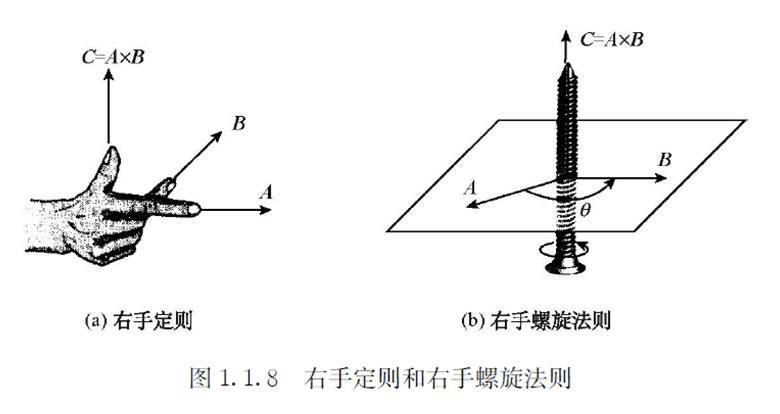
\includegraphics[width=0.65\textwidth]{img/0089.jpg}\\


\subsubsection{$\vec{b} \times \vec{a} = \vec{c}$}


1.食指朝$向\vec{b}$ 的方向. \\

\includegraphics[width=0.3\textwidth]{img/0085.png}\\

2.握拳, 食指等收回. 此时大拇指的方向, 就是 $\vec{b} \times \vec{a} = \vec{c}$ 中 $\vec{c}$ 的朝向. \\

\includegraphics[width=0.3\textwidth]{img/0086.png}

\includegraphics[width=0.65\textwidth]{img/0090.png}\\

所以, 在3D图像学中，叉乘的概念非常有用，可以通过两个向量的``叉乘"，生成第三个垂直于a，b的``法向量"，从而构建X、Y、Z坐标系. \\


\includegraphics[width=0.3\textwidth]{img/0087.png}

\includegraphics[width=0.5\textwidth]{img/0088.png}\\


~\\
\hrule
~\\












\end{document}